\section{Introducción}

En nuestros días estamos viviendo una pandemia que empezó en 2019 y sigue su crecimiento hasta día de hoy. El virus que originó este caos tanto económico como de salud pública mundial es el SARS-Cov-2, hallado en China a finales del año 2019. El SARS-Cov-2 tiene una alta tasa de contagios, lo que exige una actuación rápida para poder combatirlo. El virus afecta en mayor medida al sistema respiratorio, generando en cada persona diferentes grados de síntomas o en algunos casos hasta la muerte. Aunque, también se ha encontrado que el virus afecta a diferentes tejidos del cuerpo. Debido al gran impacto que ha generado en el mundo en todos los ámbitos, se necesita de manera urgente encontrar vacunas o medicamentos. 

\begin{figure}[h!]
			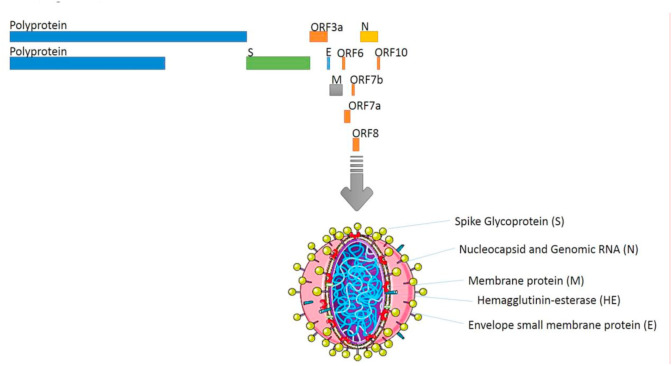
\includegraphics[width=0.9\textwidth]{figures/gr1_lrg.jpg}
			\caption{Estructura del coronavirus}
			\label{fig:cost_genome}
		\end{figure}
\newpage
		
Para la reutilización de medicamentos o de la creación de nuevos medicamentos, se necesita saber como actúa el SARS-CoV-2 durante la infección y los cambios moleculares en las proteínas humanas. Hoy en día, no hay medicamentos antivirales contra el coronavirus. Dicho anteriormente, el desconocimiento de detalles de la molécula del SARS-Cov-2, impide que se obtenga una evaluación precisa para la creación de fármacos. Esto supone un largo tiempo de investigación.

Después de ver unos cuantos artículos sobre como resuelven este problema de la reutilización del fármaco, concluimos en que la mejor estrategia es la basada en la elección de fármacos a través de la creación de una red interactoma humano perturbado por el SARS-Cov-2. A partir de ella, se verá los tejidos afectados por el virus y se priorizará los medicamentos existentes en función de las proteínas humanas y dichas interacciones. Para interrumpir el interactoma del SARS-CoV-2, buscamos ligandos de proteínas humanas que interactúen con proteínas virales. 

		
